% latex article template

% cheat sheet2(eng): http://www.pvv.ntnu.no/~walle/latex/dokumentasjon/LaTeX-cheat-sheet.pdf
% reference manual(eng): http://ctan.uib.no/info/latex2e-help-texinfo/latex2e.html

% The document class defines the type of document. Presentation, article, letter, etc. 
\documentclass[12pt, a4paper]{article}

% packages to be used. needed to use images and such things. 
\usepackage[pdfborder={0 0 0},colorlinks=true,linkcolor=blue]{hyperref}
\usepackage[utf8]{inputenc}
\usepackage[english]{babel}
\usepackage{graphicx}
\PassOptionsToPackage{hyphens}{url}

% hides the section numbering. 
% this makes \ref{marker} show up as empty. use \nameref{}, or \pageref{}
%\setcounter{secnumdepth}{-1}

% Graphics/image lications and extensions. 
\DeclareGraphicsExtensions{.pdf, .png, .jpg, .jpeg}
\graphicspath{{./images/}}

% Title or header for the document. 
\title{
	Modelling repost, IT consulting firm.\\
	TDT4252 - Enterprise Modelling and Enterprise Architecture
}
% Author
\author{
	Magnus L. Kirø \\
}
\date{\today}

\begin{document}
\maketitle
\pagenumbering{arabic}

\begin{abstract}
This is a report that covers a modelling process and its model, based on a
created case. The case is an IT consulting firm. 
%deadline: 25. april 2015 16:00 
%page limit: none, aka 20 pages. 
\end{abstract}

\tableofcontents
\newpage

%The term paper is a report that must include the following:

\section{Case description}
%A good textual description of the case that you will model and your motivations
%for selecting this case and modelling. Are there any challenges you want to
%address? Is there something you want to clarify? 

%What
The case describes an IT company, startup or existing, that has multiple
offices in Europe, is expanding, and has some form of internal structure to
assist the work the company does. For the case the name 'NewLigtning' has been
used as a working name for the company.

The IT-company has seven offices in Europe. It is currently expanding its
business and needs an overview of existing locations, culture, and main
influence flow. This is dependent on the size of the different offices and how
long the office has been in existence.

Further it is needed to clearly present the core of the company. This is the
essential strategy; the why, how and what of the company. Modelling this will
give an easy way of portraying the strategy to new consultants and potential
clients.   

For further expansion and employee satisfaction a development structure has to be
described. This should be a view that presents the different levels one can
achieve in the company, the reward at that level, and the general criteria for
each level.  

%motivations 
Motivation for this model is mostly to increase personal knowledge, but also to
be able to share this knowledge easily in the future. A big part of knowledge
sharing is the ability to understand the content and be able to boil it down to
the essential message of the knowledge. In general the value of a company have
to be understood and loved to be able to work in it an develop it further.    

% challenges to address. 
The main challenge will be to creatively create models that satisfactorily
describes a big enough portion of the company to be able to give an overview.
This is a difficult task, as there are multiple meaning of what is most
important. Another aspect is to be able to reuse the model some time in the
future. It should be so general that it could be used for a while, but at the
same time be accurate enough to be useful. 

% intended users of the model given
The intended users of the model are new recruits to a company, and clients of
the company. Mostly for educational purposes, and also to give an overview of
the company to existing employees. That said, there is no reason others can and
should not use the model to understand or develop businesses within, or
outside, the IT industry.

%Described your case.
%– Textual descriptions of your case, rationale for modelling or the purpose of
%modelling, design of the model and a discussion of the model and the modelling
%experience, how you would evaluate your model. (See also slide 6.)
%– Designed your model:
%• Who are the users?
%• What is the purpose of the model?
%• What do you want to achieve with your model?
%• How would you evaluate your model?

%What is the purpose of the model. 
The purpose of the model is to describe and clarify how an IT consulting firm
can operate. What are the core beliefs and the core processes to generate
value? This is described through different views. To understand how the
different parts of the company fits together it is important to model the
structure, activities and information flow. As well as the reward model for the
employees.    

In addition to describe the mechanisms of the company the model can also be
used to educate employees of the structure. In general which parts interacts
with which other parts, and also present the core of the strategy in a good
manner. 

As an added bonus the model serves the educational purpose that I, the modeller,
will acquire knowledge about enterprise modelling and how a consulting firm
is put together. 

%How would the model address your case?
The create model addressed the case by creating a parent model which describes
the connection and association of the different views. Then there are five sub
models that describe the most important aspects of the company structure.
Followed by three sub processes of one of the major views.  

%Design of the model 
Designing the model will be done with Archi, an open source modelling tool. The
tool will be used after sketching the views on paper. The paper sketching
serves the purpose to remove distractions and increase the creativity space,
and improve the creation process. 

% Ensure that the model meets its purpose ? 
To ensure that the model meets its purpose some evaluation criteria will be
suggested, as well as an evaluation of the modelling process. It would also be
a good idea to use peer review for the evaluation of the model. The more input
the better. The industry should ideally be involved also. 

% Were there alternative ways to do it?
There are always alternative ways to create models. Many of them not as
efficient, but some might be better. As an example of a different approach one
could use google draw or libre office draw to create the models. This approach
lacks the constraints that the Archi modelling tool gives for free. Although
the constraints of the modelling tool can limit the relations between objects.
Or there might not be an object in the modelling tool that represents the idea
in a good manner.  

\section{Model and views}
% Modelling includes conceptualising the problem as well as representing the
% concepts using an IT application or other means

% It is important that you are able describe the case, the rationale for the
% model or the purpose of the model, the design ideas, the model itself and
% your modelling experience

%Purpose of the model. as a whole. 
%Rationale for modelling or purpose of the model 
The purpose of the model as whole is to easily describe the connection of the
different parts of the business. The most important thing for any model is to
represent the intended concept in an understandable manner. See the first
section for the case related purpose of the model.

% description of the modelling tool. 
Achi was used to create the models. Archi is an open source modelling tool. 
Archi describes themselves as: "A free and open source modelling tool to create
ArchiMate models and sketches. Used by hundreds of Enterprise Architects
throughout the world.". The tool has strengths and weaknesses, but is mostly
satisfactory in terms of the outcome of the models.
Archi has folders for all the components, and a list of views. The components
are presented in views, and connected with relations. There are five categories
of modelling components; business, infrastructure, application, meta, and
other. 

% Requirements of the models. 
The model was required to include at least five perspectives of an enterprise.
Some of the suggested perspectives were: Business Processes, Actors,
Organisation and resources, Applications, Technical Systems and Requirements,
Goals or motivations, Information, and Concepts. 

When modelling an enterprise there are quite a few important aspects to think
about. These aspects can be describes as different perspectives, or rather
different ways to look at the company and how it works. Some of the enterprise
perspectives to be used, to a varying degree, is the following: Behavioral,
Functional, Structural, Goal and rule-oriented, Object oriented, (Social)
communication, Actor/role oriented, Topological. 

For the created models the perspectives in GEMAL(General Enterprise Modeling and
Activation Language) has been used for inspiration. The GEMAL perspectives are:
Goal, Process, Organisation, Product, System, Person, Capability, Location.
These perspectives are not directly modelled, but can be easily recognized in
the models where they are present.  

%Reasons for choosing these domains given, aka these specific views of the
%total model.
The split into the nine views was easy. After looking the case from different
angles, and thinking about how to best communicate the core of the company the
views became elementary. When the communication approach was defined, the
different views more or less created themselves.  

%For every model: 
%Explain why, or why not, processes, rules and
%requirements exist or do not exist
It is important to understand why, or why not, the model was created, what the
model describes, rules and requirements the affects the model, and any
processes that is described within the model. 

% intended users of each view given 
\subsection{Parent}
%* Model of models and their relations. (company overview)
Figure 1, the parent view describes the relation between different parts of the
company. Or rather the important concepts of the company.   
Each employee is a stakeholder for the well being of the company. So this view
is important for all employees to know about.  

From this view the overview of the company is the important lesson to learn. In
general, if a person do not know how the company essentially is connected that
person cannot work efficiently in it. 

\begin{figure}[htb]
    \centering
    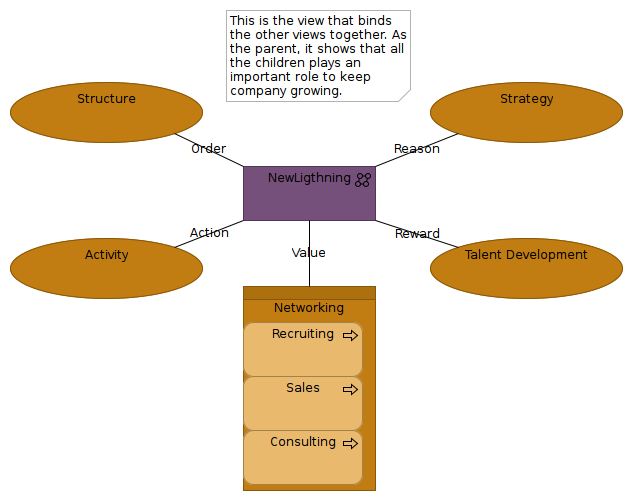
\includegraphics[width=\textwidth]{NewLightning-parent} 
    \label{fig:NewLigthning-parent}
    \caption{Parent view, showing how the other models are connected.}
\end{figure}

\subsection{Strategy}
The strategy view, figure 2, shows the vision, values and important actions to achieve the
goals of the company. The vision, values and mission is described by the why,
how and what groups. The values are linked to the inner group. This represents
that connection the more important category. 

This view should be read from the inside out. Beginning with the why, follow
with the how and finish with the what. The reason a company exists is more
important than the what and how. How is more important than what. And that
leaves the what to be the result of a good core with well established values
around it. The what if left to describe common activities that are greatly
improved by the two other categories, why and how. 

\begin{figure}[htb]
    \centering
    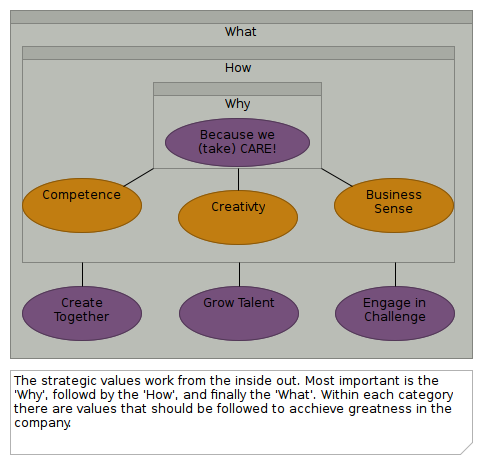
\includegraphics[width=\textwidth]{Strategy} 
    \label{fig:Strategy}
    \caption{Strategy}
\end{figure}

\subsection{Activity}
The activity view, figure 3, displays the different activities the company has to do to
create value. It shows how people are connected in the company, and which groups
of people company has. 

What this view also show is how people interact in the company. How the
information flows, and how the different roles are dependent. This view can
also be interpreted as the objects being roles. This limits the organisations
flexibility and strengthens a strong separated structure. Therefore this view
represents activities, which in turn can be performed by anyone in the company. 

\begin{figure}[htb]
    \centering
    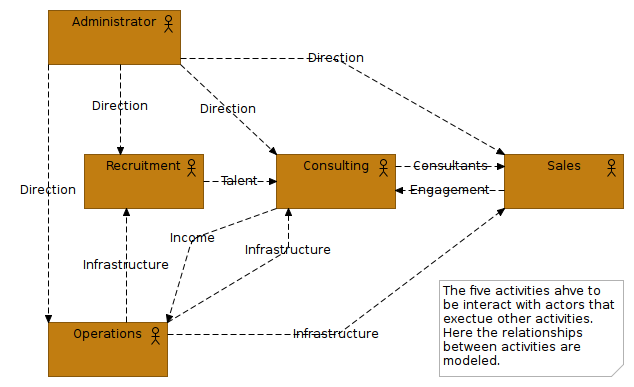
\includegraphics[width=\textwidth]{Activity} 
    \label{fig:Activity}
    \caption{Activity}
\end{figure}

\subsection{Talent Development}
The talent development model, figure 4, describes the benefits. What people are
getting, what is expected of them, and what level they are on.

Here the first stairs to the left are the consultant levels, or positions in
the company. The middle stairs are the compensation structure, and the left
stairs represent the description of the required skill and mentality of that
level.

The size of the steps on the left stairs represent the experience and
competence of the employee. 

\begin{figure}[htb]
    \centering
    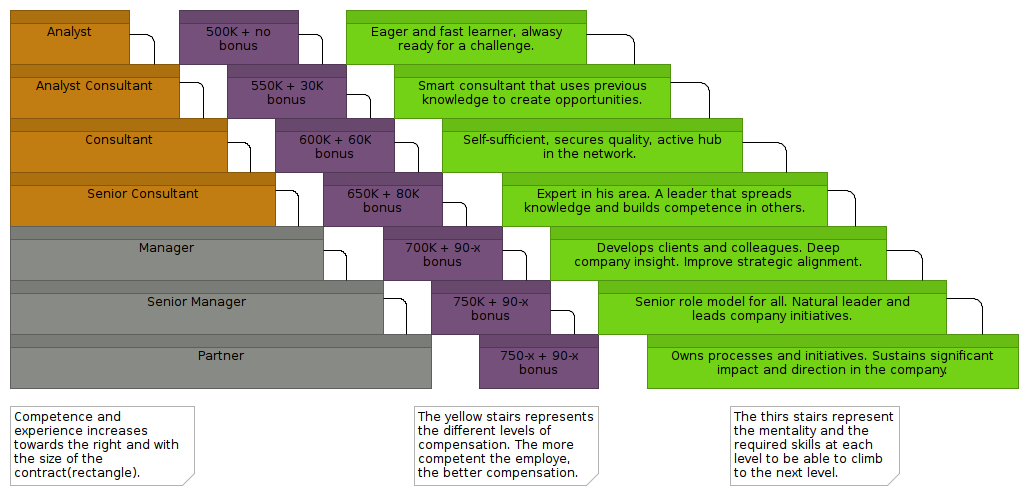
\includegraphics[width=\textwidth]{TalentDevelopment} 
    \label{fig:TalentDevelopment}
    \caption{Talent Development}
\end{figure}

\subsection{Structure}
To know the company and the resources in it there has to be some structure to
it. In figure 5, the structure view, the locations of the firm is displayed. 
It shows how the company as a whole with its international structure. 

The stairs shows in what order the offices was created, and how the expansion
developed. On the right is the cultural link between the different offices,
this is based on the difference in culture and a bit geography. 
On the right we see the main influence flow. This is how the company as a whole
is mostly influenced. Stockholm was the first office, and is the largest, along
with the central management being there it is the strongest influencer in the
company. This is important to know when considering expansion of the company,
and internal communications, culture matters.   

\begin{figure}[htb]
    \centering
    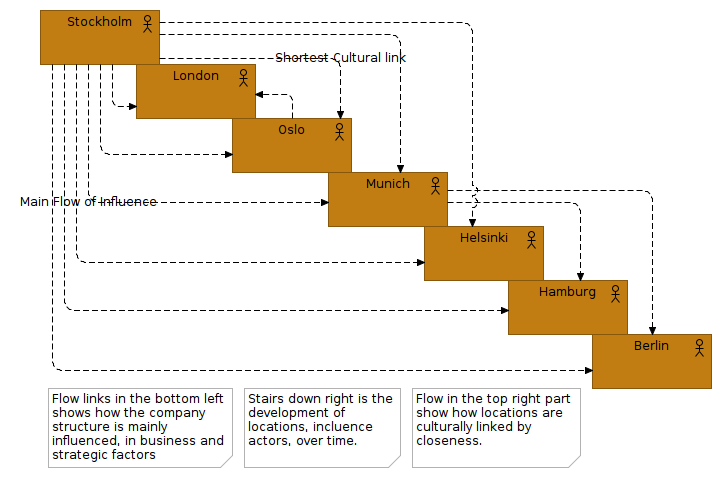
\includegraphics[width=\textwidth]{Structure} 
    \label{fig:Structure}
    \caption{Structure}
\end{figure}

\subsection{Networking}
This is in essence the combination of business processes, also known as how the
company makes money. Figure 6 shows how the networking part of the company is
organised. As a consulting firm networking is the main activity of the company.
Networking is the essence of what the business does. 

In the figure we have the networking process, with operation as the activity
that is closes to the centre of the company. This does not mean that operations
is the most important to networking, rather the opposite. Networking is best
performed at the edges of a network. This is done by the three sub processes of
operations, consulting, sales and recruitment. Operations works as support for
the three sub processes. 

\begin{figure}[htb]
    \centering
    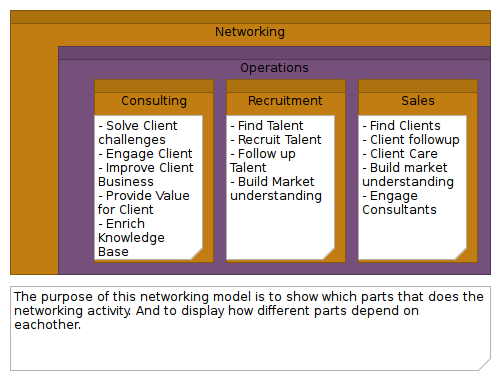
\includegraphics[width=\textwidth]{Networking(BP)} 
    \label{fig:Networking}
    \caption{Networking}
\end{figure}

\subsection{Recruiting}
Recruiting, as a sub process of the networking view, is a business process that
adds knowledge to the company. Knowledge is what the company sells, so it is
important to get new knowledge and talent all the time. 

Figure 7 shows the process of recruiting new employees. The recruiter or
possible talents can start the process. It requires two parties to continue
from the initial assessment to continue the process of employment. The process
then describes the three next states to be acquired to be rewarded with a
contract. 

\begin{figure}[htb]
    \centering
    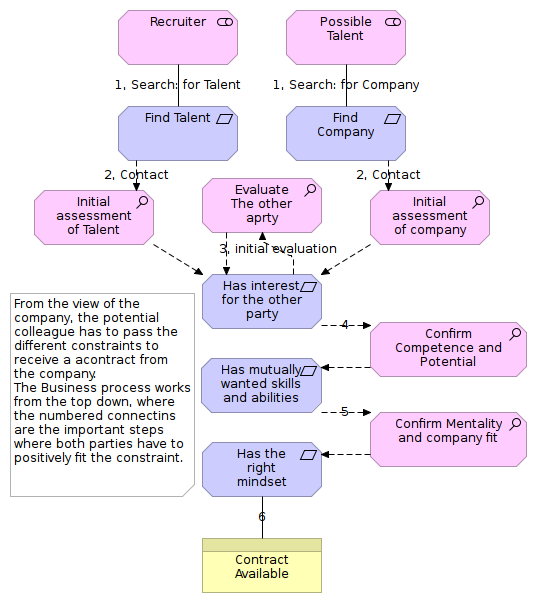
\includegraphics[width=\textwidth]{Recruitment} 
    \label{fig:Recruiting}
    \caption{Recruitment}
\end{figure}

\subsection{Consulting}
Consulting is the product that the company sells to other companies. The
essential part of consulting is to provide solutions to problems. This problem
solving process is described in figure 8.

Seven steps are used to move from the initial state of a new engagement to the
final state of a successful engagement. If the process fails at any step the
process is moved back one step and continued from there. Typically is the
evaluation step, if the plan is not good enough, a new plan is created.   

The data objects represents the association of what has been created in the
previous step, and what serves as input for the next step.  

\begin{figure}[htb]
    \centering
    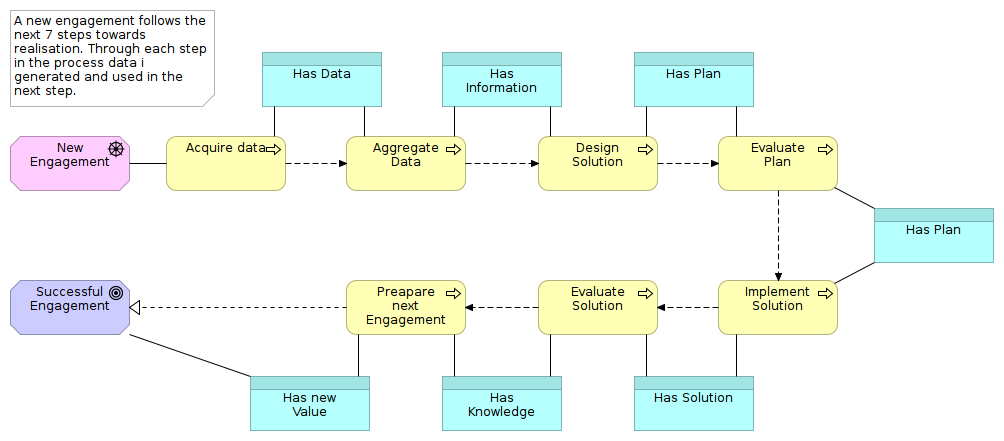
\includegraphics[width=\textwidth]{Consulting} 
    \label{fig:Consulting}
    \caption{Consulting}
\end{figure}

\subsection{Sales}
The final view is the Sales process. This business process in figure 9
describes how the company searches for and cares for clients to acquire new
engagements.  

First a client has to find the company, or the company has to find a new
client. Then the connection between client and company is assessed to find out
whether or not to commence in a relationship. When in a relationship the
company will follow up the client to assure a good relationship and possibly
prolong it. The follow up step is also there to locate new engagements.
Engagements should naturally follow good relations. 

\begin{figure}[htb]
    \centering
    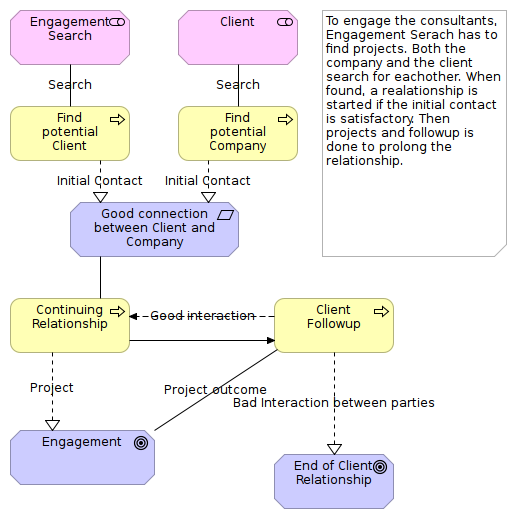
\includegraphics[width=\textwidth]{Sales} 
    \label{fig:Sales}
    \caption{Sales}
\end{figure}

\section{Perspectives explained}
%– explaining the rationale for the views (user perspective).
The different views fit into different perspectives of modelling. Following are
the touched perspectives and the views with explanation of its affiliation. 

\subsection{Business Processes}
The business perspective represents the way a company makes money, or how it is
profitable. The three sub processes of networking fits in to this perspective as
they describe how the company increases and uses its knowledge, its money
machine.

The Consulting view is business process because it show how the company
consultants solves problems, which in turn fulfils the engagement aspect of the
sales process. 

The Sales view describes how the consultant will have something to do, and
therefore create revenue. Although sales also creates knowledge, in the form of
industry understanding and market movements. Knowledge is the key capability of
the company, therefore more knowledge means more value. 

The Recruiting view shows how the company intends to acquire new talent, and
new knowledge. By having the best people the company can provide the best
services to others. Therefore is recruiting a business process that generates
value for the company.  

\subsection{Actors and Information Flow}
The activity view serves the purpose of modelling the information flow, and the
activity interaction. To assure good communication and a good flow of
information it is important to know how this works. If every one knows where to
ask the right questions the flow of information becomes easier, and more
efficient.

The activity view also serves the purpose of explaining how to adapt to the
day to day working environment. The working environment consists, roughly, of
these five actor groups. As this view can be interpreted to display three
different things(activities, roles, and departments) it is important to the
understanding of actors and information flow of the company. 

\subsection{Goals}
The goal perspective is represented through the strategy view. The strategy
view shows which values and aspects to work towards and how to achieve them. In
some ways this represents the goal of the company, in the sense that by working
towards these goals the firm will be able to achieve most other challenges in
its path.

It is important to elevate the fact that the strategy view represents the why,
how and what is necessary to achieve measurable goals for the company.
 
\subsection{Motivations}
This perspective is important to describe why people should work for the
company, and this is a major factor in what makes the company attractive to
others. A good motivational aspect of a company also increases its standing in
the industry. 

The development model, talent development, describes how employees are
rewarded, and what is the motivation on a personal level. The motivation on a
personal level represents the total motivation in the company because the
knowledge of each person aggregates to the common value of the company. This
asset then consists of the opinions, moods, and ambitions of each employee
thereby resulting in a combined motivation for the company. 
 
\subsection{Concepts}
The Networking view describes the concept that is at the core of the company.
It in many ways describe what type of company the firm is, and how it how it
should prioritise its assets to increase its value. 

The networking model, figure 6, has been inspired by
Stabell and Fjelstad, 1998 \cite{StabellFjeldstad1998}. They describe different
types of companies and three types, where networking is one of them.

\subsection{Organisation}
Structure. Parent model. 

The structure view presents the organisational perspective quite well. Here we
also have the parent model. Structure wise the view describes the international
presence of the company, which is important for people to know to understand
the global knowledge network in the company, and company's position in the
industry. 

The parent model works on a more conceptual level of the strategy,a
nd could have been placed under the Concepts perspective. Although the parent
view shows how the different views are organised and should be considered an
organisational aid. 

\subsection{Summary}
The model as a whole describes the connection of different parts of the
company, how the company operates, and the most central business processes.
Considering the purpose, easy overview and better understanding, the model as a
whole serves it purpose. The different perspectives could be better
represented, but in total its not too bad.    

\section{Model and Process evaluation}
% Describe how you evaluate your model.
%– Evaluation of the model - e.g. does the model serve its purpose?.
%How to evaluate the model
The model should be evaluated primarily by the usefulness it provides. That is
if the model preforms as intended or not. Extending this the model should be
easy to understand, and look good. Messy models will not be used in the future.
Coverage should also be an evaluating factor. Does the model cover the intended
area or concept to a satisfactory degree?

%Method,explanation
The modelling method can be described in four phases.
Initial idea, concept or sketch creation, actual modelling, and evaluation.
These four phases are all important, the actual modelling being the most
important, and the sketch/concept the most difficult one.

Modelling process
The initial idea phase is where the case, and overall modelling concept is
created. The big lines of the work. This is an easy part, because there are few
details and little logic.

The concept and sketch phase is the most difficult because it is here the logic
is created. Business logic and the logic of how to present the wanted
information in a good manner. This phase also has a tendency to overlap the
modelling phase.

The modelling phase is where the modelling tool comes into play. It is here
that all the problems with the initial concept design and sketching are
revealed and corrected. The correcting part is the reason the concept creation
and
modelling phases overlap to some degree. The modelling phase will also unveil
shortcomings in the modelling tool, which can result in recreating whole views.

Finally the evaluation phase summarises the work up to that point shortly by
stating whether or not the process has worked so far. Continuing from the
finished models the quality, coverage and compliance of the models should be
assessed. Passing these three criteria, and previously mentioned important
factors, the evaluation should result in a conclusion of whether the modelling
phase has been good.

%Explanation of the method used to evaluate the model and how the model will be evaluated

%Does it connect to purpose?
Following the description in this section we can evaluate the created model.
The purpose is served, the coverage is adequate for the purpose, but the
compliance to standards are lacking. The lack of compliance is mostly due to
lack of knowledge specifics, but also because the modelling tool has placed
restrictions on objects and relations. These restrictions has resulted in
simplifications in some views, and not using intended relations between objects
because of the lack of appropriate objects or relations. 

Summarised evaluation; The model is OK, but it could also be a lot better. In
the end it serves its purpose. 

As for the process it has been quick when first started. The idea phase was
easy and quickly followed by the concept phase. The concept phase was a bit
difficult, but ultimately work out with some time and extra thought. It is not
easy to find good ways to represent data in an intuitive manner. The
modelling phase proved a bit more tricky because of the restrictions on the
modelling tool. As for the evaluation process it is difficult to say anything
about it due to lack of experience with modelling and evaluation of models. The
models seem fine, but it is difficult to say what others would think. 

Process in total; As expected, some problems along the way, but mostly easy
going with a satisfying result.  

\section{Relation to Enterprise Architecture(EA)}
– Discuss how your model can be used to support Enterprise Architecture.
Lessons learned

The relation to enterprise architecture this model is inadequate. Technology
and changes are not thoroughly addressed. This is because of the scope of the
case. The case is limiting, and therefore the model is limited. On the other can
this model can be expanded to contain missing parts of an EA approach.

If we only consider how the created model can be used to assist in EA the model
is not bad. But it could be improved greatly. The fact that the created model
is based on a company as a case it already has a lot of EA elements, such as
information flow, motivation, strategy, and structure.

Through the modelling elements of EA and Enterprise modelling has been learned,
and improvements to conceptualisation and modelling abilities has acquired. Key
modelling pointers are to keep it simple, use what is available, and use
comments. Relations are not always easy to describe and there are a lot of
relations a tool is not adequate to present. Also learned: to use Archi. 

\section{Business Model}
%– Create a business model for your enterprise, using Business Modelling,Canvas.
%describe how the model is a business case and how it can be used in a business
%situation. 

To describe a model in a business relation is important. The essence of a
business model is to be able to clearly present the value the model brings to
the table. If the model has no value it can not be described as a business
model.   

%business case
The created model is based on a case that is intended to be a business. This
greatly influences the model to become a business model. By looking at the
different applications and potential use cases for the model it can clearly be
categorised as a business model. Most important from the created model is the
strategy and business processes(the processes to generate revenue).   

%how used in business.
For use cases in business the created model is adequate to describe the
strategy and structure of the case company. It also describes the flow of
information within the company and the development system. The model is
constructed to be used in these cases. Additionally the parent model, showing
how the other models are connected, is useful in a business relation, for
presenting the connection of strategic parts of the company. The easier it is
for people to understand how the system in a company works, the better.   

\section{Discussion and Reflection}
% Discussion and reflections – lessons learned
%– Reflections about your modelling exercise: the modelling process that you have
%been through, lessons learned. 

The process as a whole has resulted in the inevitable last minute rush, the
result is according. Although the result is adequate considering the time
spent. The knowledge gained is substantial, and the experience in modelling is
much better than before. 

As for the subject, it is important and useful. Although might be boring most
of the time. The task should also be more rigorously structured. Different
chunks with defined deliveries and deadlines. This forces participants to
deliver smaller parts more often, take inspiration from agile. 

%Discussion of possible evaluation methods 
For possible evaluation methods on should prefer peer review. This is the
standard evaluation method for science. But this method is rather slow.
Solutions such as an expert panel should be explored. That is more efficient,
and might give better results. Although this will not give a good insight into
the understandability of the model. Ten people might understand the model just
fine, while the one evaluating it might not, here we have a good model and a
bad evaluator. The opposite might also be the case. 

% Evaluation of the model in relation to the intended purpose 
The model has its good and bad sides. Use cases described in the previous
section are a good example of how the model is versatile, and good. But the
quality of the model is unknown, which is bad. In total the model is sufficient
for its purpose, to better understand a potential structure and inner workings
of a company. 

% report
For the report there are a few keywords to be used; fast and concrete. There
are no unnecessary content in the report, or at least that is the intention.
Most requirements are covered, but most of them could be elaborated a lot more. 
All in all the work is sound, but not perfect. The working method has been
based on the thoroughly tested 'just get it done' method, where perfection is
set aside and getting results are in focus.  


% references / bibliography
%\cite{deyer}
\addcontentsline{toc}{section}{References}
\begin{thebibliography}{1}
%\bibitem{deyer}{
%Dyer, J. H., Kale, P., & Singh, H. (2001). Strategic alliances work. MIT Sloan
%Management Review, 37-43.
%}

\bibitem{StabellFjeldstad1998}{
Configuring Value for Competitive Advantage: On Chains, Shops And Networks.
CHARLES B. STABELL* and ØYSTEIN D. FJELDSTAD,
Norwegian School of Management, Sandvika, Norway.
Strategic Management Journal, Vol. 19, 413–437 (1998)
}

\end{thebibliography}

% alternatively, if big bibliography
%\bibliographystyle{abbrv}
%\bibliography


\end{document}
This is never printed
